% This file makes a printable version of the blueprint
% It should include all the \usepackage needed for the pdf version.
% The template version assume you want to use a modern TeX compiler
% such as xeLaTeX or luaLaTeX including support for unicode
% and Latin Modern Math font with standard bugfixes applied.
% It also uses expl3 in order to support macros related to the dependency graph.
% It also includes standard AMS packages (and their improved version
% mathtools) as well as support for links with a sober decoration
% (no ugly rectangles around links).
% It is otherwise a very minimal preamble (you should probably at least
% add cleveref and tikz-cd).

\documentclass[letter]{report}

\usepackage{geometry}

\usepackage{expl3}

\usepackage{amssymb, amsthm, mathtools}
\usepackage[unicode,colorlinks=true,linkcolor=blue,urlcolor=magenta, citecolor=blue]{hyperref}

\usepackage[warnings-off={mathtools-colon,mathtools-overbracket}]{unicode-math}

%\usepackage{times}

% In this file you should put all LaTeX macros and settings to be used both by
% the pdf version and the web version.
% This should be most of your macros.

% The theorem-like environments defined below are those that appear by default
% in the dependency graph. See the README of leanblueprint if you need help to
% customize this. 
% The configuration below use the theorem counter for all those environments
% (this is what the [theorem] arguments mean) and never resets it.
% If you want for instance to number them within chapters then you can add
% [chapter] at the end of the next line.
\newtheorem{theorem}{Theorem}[chapter]
\newtheorem{proposition}[theorem]{Proposition}
\newtheorem{lemma}[theorem]{Lemma}
\newtheorem{corollary}[theorem]{Corollary}

\theoremstyle{definition}
\newtheorem{definition}[theorem]{Definition}
\newtheorem*{theorem*}{Theorem}
\theoremstyle{remark}
\newtheorem{remark}[theorem]{Remark}


\newcommand{\TT}[2]{T_{2^{#1}}\left(#2\right)}
\newcommand{\threesevenths}{\frac{3}{7}}
\newcommand{\offset}{\frac{8^{-k}}{14}}
\newcommand{\halfsum}[3]{\frac{1}{2} \sum\limits_{m = #1}^{#2} 8^{-m} \TT{m}{#3}}
\newcommand{\dotpsi}[2]{\dot{\psi}_{#1}\left(#2\right)}
\newcommand{\ddotpsi}[2]{\ddot{\psi}_{#1}\left(#2\right)}


% In this file you should put macros to be used only by
% the printed version. Of course they should have a corresponding
% version in macros/web.tex.
% Typically the printed version could have more fancy decorations.
% This should be a very short file.
%
% This file starts with dummy macros that ensure the pdf
% compiler will ignore macros provided by plasTeX that make
% sense only for the web version, such as dependency graph
% macros.


% Dummy macros that make sense only for web version.
\newcommand{\lean}[1]{}
\newcommand{\discussion}[1]{}
\newcommand{\leanok}{}
\newcommand{\mathlibok}{}
\newcommand{\notready}{}
% Make sure that arguments of \uses and \proves are real labels, by using invisible refs:
% latex prints a warning if the label is not defined, but nothing is shown in the pdf file.
% It uses LaTeX3 programming, this is why we use the expl3 package.
\ExplSyntaxOn
\NewDocumentCommand{\uses}{m}
 {\clist_map_inline:nn{#1}{\vphantom{\ref{##1}}}%
  \ignorespaces}
\NewDocumentCommand{\proves}{m}
 {\clist_map_inline:nn{#1}{\vphantom{\ref{##1}}}%
  \ignorespaces}
\ExplSyntaxOff

\title{Formalizing a Lipschitz continuous version of Kolmogorov's superposition theorem}
\author{Ben Goodrich}

\begin{document}
\maketitle
% In this file you should put the actual content of the blueprint.
% It will be used both by the web and the print version.
% It should *not* include the \begin{document}
%
% If you want to split the blueprint content into several files then
% the current file can be a simple sequence of \input. Otherwise It
% can start with a \section or \chapter for instance.

\chapter{Introduction}

This project is not yet complete, but intends to formalize a strengthening of the following theorem. Let $\mathbb{I} = \left[0,1\right]$ and let $n \geq 2$ be an given integer. We use $C^d$ to indicate the space of functions defined on a domain whose $d$-th derivative is continuous and use $\circ$ to indicate function composition.

\begin{theorem*}[Kolmogorov 1957]
  \label{thm:KST}
  For every $f \in C\left(\mathbb{I}^n\right) \mapsto \mathbb{R}$, there exist increasing $\psi_{p,q} \in C\left(\mathbb{I}\right) \mapsto \mathbb{R}$ that do not depend on $f$ and generally non-monotone $\chi_q \in C\left(\mathbb{R}\right) \mapsto \mathbb{R}$ that depend on $f$ and $\psi_{p,q}$, such that $f\left(x_0, x_1, \cdots, x_{n - 1}\right) = \sum\limits_{q = 0}^{2n} \chi_q \circ \Psi_q\left(x_0, x_1, \cdots, x_{n - 1}\right)$, where $\Psi_q\left(x_0, x_1, \cdots, x_{n - 1}\right) \equiv \sum\limits_{p = 0}^{n - 1} \psi_{p,q}\left(x_p\right)$.
\end{theorem*}

\noindent This theorem is called the Kolmogorov Superposition Representation (KSR) or the Kolmogorov Superposition Theorem (KST) because Kolmogorov proved that a given multivariable ``target'' function, $f$, could be represented as a finite sum of compositions of univariate functions. 

The relevance of the KRT continues to be debated in the neural networks literature. On one side, many want to utilize the KSR to approximate unknown or expensive target functions. However, the ``inner'' functions, $\psi_{p,q}$, and ``outer'' functions, $\chi_q$, are not elementary, in the sense that they cannot be computed with a finite number of calls to basic functions. Thus, the KSR requires harmonic analysis and other side is skeptical that the it will ever be of much practical use.

Although the KST is perhaps surprising in its generality and simplicity, it has been proven in several ways, raising the question of what value is added by an additional proof? The extant proofs of the KST are of three kinds (and none have been formalized):

\begin{itemize}
    \item \textbf{Nonconstructive}: The most elegant proofs utilize the Baire Category Theorem to prove the \textit{existence} of inner and outer functions that satisfy the KST but do not suggest how to construct them.
    \item \textbf{Constructive}: Other proofs are considered to be constructive but do not even suggest a feasible algorithm to implement them in floating-point arithmetic.
    \item \textbf{Constructed}: Two constructions have been implemented in software but both utilize bad inner functions and worse outer functions, making them unworkable in floating-point arithmetic.
\end{itemize}

By ``bad" inner functions, we specifically mean they are in the Devil's Staircase family, that is, their derivative is zero almost everywhere on $\mathbb{I}$ but does not exist on a dense set of points. By ``worse" outer functions, we specifically mean that they are nowhere differentiable. Thus, even if $f$ were differentiable at some point, the chain rule does not apply to a compositions involving nowhere differentiable functions, so it cannot be used to compute a gradient under the original KSR. Most algorithms in statistics and supervised learning rely on gradients as part of some larger algorithm, so the KSR has not been useful for those purposes. 

Our goal is to construct decent inner functions and adequate outer functions that satisfy the KST and allow the chain rule to compute the gradient of $f$, which can then be implemented to floating-point arithmetic. Vitushkin and Khenkin proved that the inner functions in the KST cannot all be continuously differentiable. Thus, by ``decent'' inner functions, we specifically mean Lipschitz continuous functions, which satisfy $\left|\psi_{p,q}\left(x\right) - \psi_{p,q}\left(x^\prime\right)\right| \leq K\left|x - x^\prime\right|$ for some positive but finite constant $K$. The KST literature often refers to a more general definition of Lipschitz continuity (which is also termed H\"{o}lder continuity) where $\left|\psi_{p,q}\left(x\right) -   \psi_{p,q}\left(x^\prime\right)\right| \leq K\left|x - x^\prime\right|^\alpha$. Fridman and Kahane proved that the inner functions can all be weak contractions, that is, $\alpha = 1$ and $K = 1$.

Sprecher proved that there are outer functions that satisfy the KST for any target function when $\psi_{p,q}\left(x_p\right) \equiv \lambda^p \varphi\left(x_p - \frac{q}{2n}\right)$, where $\lambda > 0$ is an irrational number and $\varphi$ is a weak contraction that we call the ``core'' function. However, the only known attempt to implement the Fridman-Sprecher approach in software was made by Actor, which was unsuccessful.

Actor did succeed in reparameterizing the H\"{o}lder continuous core function proposed by Sprecher, corrected by K\"{o}ppen, and proven correct by Braun and Griebel. Actor's function is parameterized via its arc length and is Lipschitz continuous by construction. While there is graphical evidence that strongly suggests Actor's function is compatible with the KST, some aspects of the approach are not fully proved, and it requires an expensive numerical inversion of Braun and Griebel's function just to achieve a few decimal places of accuracy.

Montanelli and Yang notes the importance of constructing a Lipschitz continuous KST
\begin{quote}
We have proven upper bounds for the approximation of multivariate functions $f : [0, 1]^n \mapsto \mathbb{R}$ by deep ReLU networks, for which the curse of dimensionality is lessened. The depth and the size of the networks to approximate such functions $f$ grow like $\mathcal{O}\left(\varepsilon^{-\log n}\right)$, as opposed to $\mathcal{O}\left(\varepsilon^{-n}\right)$. The proof is based on the ability of very deep ReLU networks to implement the Kolmogorov-Arnold superposition theorem.

There are many ways in which this work could be fruitfully continued. If we were able to construct a Lipschitz continuous inner function, we would be able to
obtain $\mathcal{O}\left(\varepsilon^{-1}\right)$ estimates. Actor and Knepley designed in 2017 an algorithm to compute a Lipschitz continuous inner function, but they did not provide a method to compute the outer functions.
\end{quote}
\noindent This quote reflects the fact that the outer functions depend on the inner functions, in addition to $f$. The smoother are the inner functions, the easier it is to obtain ``adequate'' outer functions that approximate a target function to a given degree of accuracy. In short, a Lipschitz continuous KST would overcome (to first order) the curse of dimensionality when approximating $y$ on $\mathbb{I}^n$. 

Also, target functions in statistics, such as log-likelihood functions, typically depend on $N$ data points and the cost of evaluating them directly is polynomial (at best) in $N$. Once the outer functions have been calibrated to the target function, the KSR of the target function can be evaluated in parallel in essentially constant wall time regardless of $n$ or $N$. These savings could be enormous in computationally intensive applications, such as Markov Chain Monte Carlo or Large Language Models.

There are several open questions that are not even investigated in the KST literature:
\begin{enumerate}
    \item Can some proper subset of the inner functions be continuously differentiable (or smoother)? We show that if $0 < q < 2n$, then $\psi_{p,q}$ can be twice continuously differentiable.
    \item Does the core function depend on $n$, apart from being evaluated at $x - \frac{q}{2n}$? We show that $\varphi$ can be universal, although $\lambda$ does depend on $n$ in a simple fashion.    
    \item Can the set of points where $\varphi$ is not differentiable be finite? We show that $\varphi$ is not differentiable at $1$ and $-1$ but is differentiable on $\left(-1,1\right)$.
    \item Can $\varphi$ be approximated to floating-point precision? We show that $\varphi$ can be quickly approximated to any degree of accuracy. 
\end{enumerate}

Our approach is unique in that we first construct a function with the requisite properties and then show that it is a viable core function in the KSR. Chapter \ref{ch:CoreFunction} uses basic real analysis --- most of which is already formalized in the Mathlib library used by the Lean software --- to show that our candidate for $\psi$ is increasing, Lipschitz continuous, and not continuously differentiable. In addition, since $\varphi$ can be represented as a series, it is essential to demonstrate that the series converges uniformly, which is an improvement over the other constructions in the KST literature whose functions only converge pointwise. As a result, $\varphi$ can be evaluated to double precision in fewer than a hundred floating point operations, and its derivative can be evaluated at double that cost (albeit to less accuracy).

Chapter \ref{ch:Injectivity} establishes in Lean that $\Psi_q\left(x_0, x_1, \cdots, x_{n - 1}\right) \equiv \sum\limits_{p = 1}^n \lambda^{p -1} \varphi\left(x_p - \frac{q}{2n}\right)$ is injective for each $q$ when $\lambda$ is a transcendental number. The proof is only slightly different from the one Sprecher has relied upon for decades that essentially extended the rational number field with an irrational $\lambda$. Much of this can leverage the theorems on cyclotomic fields that are already in Mathlib.

Chapter \ref{ch:OuterFunctions} is the least complete but is devoted to the outer functions in the KSR. Kahane utilized the notion of a Helson set, which is a subset with the characterizing property that every continuous function over this subset can be represented as a convergent Fourier series. Kahane proved necessary and sufficient conditions for a subset of $\mathbb{I}^{2n + 1}$ to be a Helson set.

\chapter{Core Function}\label{ch:CoreFunction}

\section{Main Definitions}\label{sec:MainDefinitions}

The atomic element of our KSR is the first-kind Chebyshev polynomial. Let $j$ be a generic integer that is usually non-negative, but is used in various ways in different contexts in this report.
\begin{definition}[Chebyshev polynomial of the first kind]
  \label{def:T}
  \leanok
  Let $r$ be a real number. The first-kind Chebyshev polynomial in $r$ with index $j$ is defined via a three-term recursion as
  \begin{align*}
T_j\left(r\right) \equiv 
\begin{cases}
1 & \text{if } j = 0 \\
r & \text{if } j = 1 \\
2 r T_{j - 1}\left(r\right) - T_{j - 2}\left(r\right) & \text{if } j > 1.
\end{cases}
  \end{align*}
\end{definition}
\begin{remark*}
The Mathlib library used by Lean (version 4) actually defines $T_j$ as a function of $j$ (which can be negative) that returns a polynomial (with coefficients in any commutative ring). Such generality is unnecessary here, but Mathlib also provides a metatheorem that can be used to tersely prove many properties of Chebyshev polynomials via double induction on $j$. Our notation, $T_j\left(r\right)$, corresponds to simply evaluating such a polynomial at a symbolic real number. 
\end{remark*}
We specialize $j = 2^m$ to define partial sums that approach our candidate for a core function.
\begin{definition}[$k$-th order approximator]
  \label{def:approx}
  \uses{def:T}
  \leanok
  $\varphi_k\left(r\right) \equiv \threesevenths + \offset + \halfsum{0}{k}{r}$, where $k \in \mathbb{N}$.
\end{definition}
\begin{definition}[Core function]
  \label{def:core}
  \uses{def:T}
  \leanok
  $\varphi\left(r\right) \equiv \threesevenths + \halfsum{0}{\infty}{r}$.
\end{definition}
\noindent For an overview of expanding a function in terms of Chebyshev polynomials, see Trefethen.

\begin{definition}[Normalizer]
  \label{def:Lambda}
  $\Lambda \equiv \sum\limits_{p = 0}^{n - 1} \lambda^p$, where $\lambda > 0$ and $n \geq 2$.
\end{definition}
\begin{definition}[Scale factor]
  \label{def:lambda_p}
  \uses{def:Lambda}
  $\lambda_p \equiv \frac{\lambda^p}{\Lambda} \in \left(0,1\right)$.
\end{definition}
\begin{definition}[Inner function]
  \label{def:inner_function}
  $\psi_{p,q}\left(x\right) \equiv \lambda_p \varphi\left(x - \frac{q}{2n}\right)$, where $x \in \mathbb{I}$ and $q \in \{0, 1, \cdots, 2n\}$.
\end{definition}

\section{Repeatedly Used Lemmas}\label{sec:RepeatedlyUsedLemmas}

\renewcommand{\thetheorem}{\Alph{theorem}}

Our Chebyshev polynomials also follow a \emph{two-term} recursion that drives nearly all other lemmas.
\begin{lemma}[Two-term recursion]
  \label{lem:TT_recursion}
  \uses{def:T}
  \lean{TT_recursion}
  \leanok
  $\TT{m + 1} = 2\TT{m}^2 - 1$, where $m \in \mathbb{N}$.
\end{lemma}
  
\begin{proof}
  \leanok
  Since $2^{m + 1} = 2 \times 2^m$, we can write $\TT{m + 1} = T_{2 \times 2^m}$. It is already proven by induction in Mathlib (TODO: add succinct explanation) that a Chebyshev polynomial whose index is a product of integers can be written as a composition of two Chebyshev polynomials, so $T_{2 \times 2^m} = T_2 \circ \TT{m}$. It follows from Definition \ref{def:T} that $T_2\left(r\right) = 2r^2 - 1$, so $T_2 \circ \TT{m} = 2\TT{m}^2 - 1 = \TT{m + 1}$.
\end{proof}

\begin{lemma}[Bounds]
  \label{lem:bounds}
  $\TT[r]{m}^2 \leq 1$ if and only if $r^2 \leq 1$.
\end{lemma}
\begin{proof}
  Since $\TT[r]{0} = r$, having $r^2 \leq 1$ is necessary and sufficient when $m = 0$. Assume it holds for $m$, so that we can use Lemma \ref{lem:TT_recursion} to show it then holds for $\TT[r]{m + 1}^2 = \left(2\TT[r]{m}^2 - 1\right)^2$. Under the inductive hypothesis that $\TT[r]{m}^2 \leq 1$, then the entire right-hand side is less than one in magnitude. Conversely, if $\TT[r]{m}^2 > 1$, then the right-hand side remains greater than one in magnitude.
\end{proof}

\begin{lemma}[Fixed points]
  \label{lem:fixed_points}
  \lean{fixed_points}
  \uses{lem:TT_recursion}
  \leanok
  The only two fixed points of $2 \TT[r]{m}^2 - 1 \mapsto \TT[r]{m + 1}$ are $-\frac{1}{2}$ and $1$.
\end{lemma}

\begin{proof}
  \leanok
  If $\TT[r]{m + 1} = \TT[r]{m}$ under Lemma \ref{lem:TT_recursion}, then a quadratic equation, $2 \TT[r]{m}^2 - \TT[r]{m} - 1 = \left(2\TT[r]{m} + 1\right)\left(\TT[r]{m} - 1\right)  = 0$ whose only two solutions are $-\frac{1}{2}$ and $1$ defines the fixed points.
\end{proof}
\begin{remark*}
Both fixed points are repellent because the derivative of the mapping at a fixed point greater in magnitude than $1$. However, this has not been formalized yet since it is not a priority.
\end{remark*}
\noindent If either fixed point is reached, the remaining terms in $\varphi_k$ become a partial geometric series.
\begin{lemma}[Partial geometric series]
  \label{lem:geom_sum_neg_pow}
  If $b > 1$, then $\sum\limits_{m = j}^k b^{-m} = \frac{b^{1 - j} - b^{-k}}{b - 1}$.
\end{lemma}
\begin{proof}
  \leanok
  $\sum\limits_{m = j}^k b^{-m} = \sum\limits_{m = j}^k \left(\frac{1}{b}\right)^m \equiv S$, which is in the usual form of a geometric series with a ratio of $\frac{1}{b}$ whose partial sums are already proven in Mathlib. The usual method of proof is to note that since $S - \frac{1}{b} S = \sum\limits_{m = j}^k \left[\left(\frac{1}{b}\right)^m - \left(\frac{1}{b}\right)^{m + 1}\right] = \left(\frac{1}{b}\right)^j - \left(\frac{1}{b}\right)^{k + 1}$, then $S = \frac{\left(\frac{1}{b}\right)^j - \left(\frac{1}{b}\right)^{k + 1}}{1 - \frac{1}{b}} = \frac{b^{-j} - b^{-k - 1}}{\frac{b - 1}{b}} = \frac{b^{1 - j} - b^{-k}}{b - 1}$.
\end{proof}
\begin{lemma}[Linearly shifted sum-of-squares]
  \label{lem:SOS}
  $\varphi_k\left(r\right) = \frac{5}{14} + \frac{8^{-k}}{7} + \frac{r}{2} + \frac{1}{8} \sum\limits_{m = 0}^{k - 1} 8^{-m} \TT[r]{m}^2$. 
\end{lemma}
\begin{proof}
  Pull the $\TT[r]{0} = r$ term out of the series in Definition \ref{def:approx} and then shift the index of the summation while applying Lemma \ref{lem:TT_recursion} to all the remaining terms to obtain $\varphi_k\left(r\right) = \threesevenths + \offset + \frac{r}{2} + \frac{1}{2} \sum\limits_{m = 0}^{k - 1} 8^{-\left(m + 1\right)} \left(2 \TT[r]{m}^2 - 1\right) = \threesevenths + \offset + \frac{r}{2} + \frac{1}{8} \sum\limits_{m = 0}^{k - 1} 8^{-m} \TT[r]{m}^2 - \frac{1}{16} \sum\limits_{m = 0}^{k - 1} 8^{-m}$. Apply Lemma \ref{lem:geom_sum_neg_pow} with $b = 8$ to the last term and simplify the constant to obtain the result.
\end{proof}

\renewcommand{\thetheorem}{\thesection.\arabic{theorem}}

\section{Convergence}\label{sec:Convergence}

Let $\mathbb{T} = \left[-1,1\right]$. The infinite sum in the definition of $\varphi$ converges uniformly to \emph{some} function on $\mathbb{T}$, although it is \underline{not yet known} whether it can be written in terms of special functions. 

\begin{lemma}[]
  \label{lem:summable}
  \uses{def:core}
  \lean{ψ_summable}
  \leanok
  $\sum\limits_{m = 0}^\infty 8^{-m} \TT[t]{m}$ is summable if and only if $t \in \mathbb{T}$.
\end{lemma}
  
\begin{proof}
  \uses{lem:TT_recursion, lem:geom_sum_neg_pow}
  \leanok
  To prove the if direction, we utilize the Weierstrass M-test. Lemma \ref{lem:bounds} implies $\TT[t]{m} \in \mathbb{T}$. Since $\left|8^{-m} \TT[t]{m}\right| \leq 8^{-m}$ and $\sum\limits_{m = 0}^\infty 8^{-m} = \frac{8}{7}$ by Lemma \ref{lem:geom_sum_neg_pow} with $b = 8$, $\varphi$ is well-defined on $\mathbb{T}$.

  To prove the only if direction, we utilize the direct comparison test. It suffices to show that if $\left|t\right| > 1$, then the limit of $8^{-m} \frac{\TT[t]{m}}{8^{m}}$ as $m \uparrow \infty$ is not zero. When $\left|r\right| > 1$, it is well-known that $T_j\left(r\right) = \frac{\left(r + \sqrt{r^2 - 1}\right)^j + \left(r - \sqrt{r^2 - 1}\right)^j}{2}$, although it is not yet proven in Mathlib. We only need to prove it when $j = 2^m$, in which case if $m = 0$, then $\frac{\left(t + \sqrt{t^2 - 1}\right)^1 + \left(t - \sqrt{t^2 - 1}\right)^1}{2} = t = \TT[t]{0}$. Assuming this relationship holds for $m$ and using Lemma \ref{lem:TT_recursion} with the inductive hypothesis, we need to show that 
  \begin{eqnarray*}
  \TT[t]{m + 1} &=& 
  2 \left(\frac{\left(t + \sqrt{t^2 - 1}\right)^{2^m} + \left(t - \sqrt{t^2 - 1}\right)^{2^m}}{2}\right)^2 - 1 \\ &=&
  \frac{\left(t + \sqrt{t^2 - 1}\right)^{2^{m + 1}} + \left(t - \sqrt{t^2 - 1}\right)^{2^{m + 1}}}{2} +
  \left[\left(t + \sqrt{t^2 - 1}\right) \left(t - \sqrt{t^2 - 1}\right)\right]^{2^m} - 1 \\ &=&
  \frac{\left(t + \sqrt{t^2 - 1}\right)^{2^{m + 1}} + \left(t - \sqrt{t^2 - 1}\right)^{2^{m + 1}}}{2},
  \end{eqnarray*}
  where the last line follows from the fact that $\left(t + \sqrt{t^2 - 1}\right) \left(t - \sqrt{t^2 - 1}\right) = t^2 + 0 - t^2 + 1 = 1$. Thus, if $\left|t\right| > 1$, then $\TT[t]{m + 1} > t^{2^{m + 1}}$, which diverges at a doubly exponential rate as $m \uparrow \infty$. Since $8^{-m}$ converges to zero at a geometric rate, 
  $8^{-m} \frac{\TT[t]{m}}{8^{m}}$ diverges as $m \uparrow \infty$.
\end{proof}

Although the theoretical analysis in Lean pertains to $\varphi$, in numerical work we can only approximate $\varphi\left(t\right)$ with $\varphi_k\left(t\right)$ using floating-point numbers, so the approximation must converge rapidly.
\begin{lemma}[]
  \label{lem:limit}
  \uses{def:approx}
  As $k \uparrow \infty$, $\varphi_k$ converges uniformly to $\varphi$ on $\mathbb{T}$.
\end{lemma}
\begin{proof}
  \uses{lem:TT_recursion}
  Similarly to Lemma \ref{lem:summable}, $\left|\halfsum{0}{\infty}{t} - \halfsum{0}{k}{t}\right| \leq \frac{1}{2} \sum\limits_{m = k + 1}^\infty \left|8^{-m}\TT[t]{m}\right| \leq \frac{1}{2} \sum\limits_{m = k + 1}^\infty 8^{-m} = \offset$ by Lemma \ref{lem:geom_sum_neg_pow}. As $k \uparrow \infty$, this bound approaches $0$, so $\lim\limits_{k \uparrow \infty}\varphi_k \rightarrow \varphi$ over $\mathbb{T}$.
\end{proof}
\begin{remark*}
Since the error in approximating $\varphi\left(t\right)$ with $\varphi_k\left(t\right)$ is less than $\frac{2^{-3k}}{14}$, the approximation error if $k = 17$ is less than $\frac{2^{-52}}{7}$, where $2^{-52}$ is the smallest double-precision number that can be added to $1$ without underflow. Thus, only $18$ iterations of an unrolled loop with only a few floating-point operations per iteration are needed to evaluate $\varphi_{17}\left(t\right)$ from Lemma \ref{lem:SOS}.
\end{remark*}
\begin{remark*}
  If $t = \frac{a}{b}$ where $a \in \mathbb{Z}$ and $b \in \mathbb{N}$ such that $\left|a\right| < b$ and $a$ has no common factor with $b$, then $\varphi_k\left(\frac{a}{b}\right)$ is also rational because the only operations in Definition \ref{def:core} are arithmetic. However, $\varphi\left(\frac{a}{b}\right)$ is generally irrational but may well be algebraic rather than transcendental. Although the partial sums converge uniformly with an error bound proportional $\frac{1}{8^{-k}}$, they do so with denominators that are too large for $\varphi\left(\frac{a}{b}\right)$ to be a Liouville number. In addition, if $\TT[\frac{a}{b}]{m}$ is never either of the fixed points from Lemma \ref{lem:fixed_points}, then the numerators of the partial sums do not have a limit.
\end{remark*}


\begin{proposition}[]
  \label{prop:q=0}
  \uses{def:core}
  If $q = 0$ or $q = 2n$, then $\psi_{p,q} \notin C^1\left(\mathbb{I}\right)$.
\end{proposition}
  
\begin{proof}
  \uses{lem:TT_recursion}
  The derivative is defined as $\dot{\psi}_{p,q}\left(x\right) \equiv \lim\limits_{h \rightarrow 0} \frac{\psi_{p,q}\left(x + h\right) - \psi_{p,q}\left(x\right)}{h}$ where $\psi_{p,q}\left(x\right) \equiv \lambda_p \varphi\left(x - \frac{q}{2n}\right)$ from Definition \ref{def:inner_function}. Per Lemma \ref{lem:summable}, if $x + h - \frac{q}{2n} \notin \mathbb{T}$, then the two-sided limit in the definition of $\dot{\psi}_{p,q}\left(x\right)$ does not exist at that point. If $h > 0$, that exceptional case can occur if and only if both $x = 1$ and $q = 0$, and if $h < 0$, it can also occur if and only if both $x = 0$ and $q = 2n$.
\end{proof}
\begin{remark*}
Hence, our candidate for a core function narrowly avoids the fact proven by Vituskin and Khenkin that the KST would not hold if \emph{all} the inner functions were continuously differentiable.     
\end{remark*}

\section{Requisite Properties}\label{sec:RequisiteProperties}

\begin{figure}
    \begin{center}
    \caption{The (well-approximated) core function and its derivative}
    \label{fig:core}
    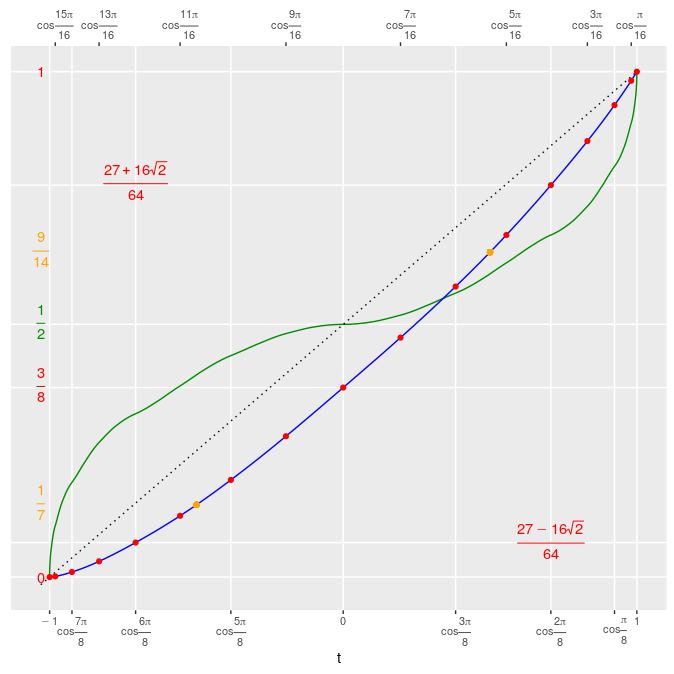
\includegraphics[width=0.95\linewidth]{../images/core.png}
    \end{center}
    \emph{The blue line is for $\varphi_{17}$, which approximates $\varphi$ to double-precision. The green line is for the exact derivative of $\varphi_{17}$, which approximates the derivative of $\varphi$ on $\left(-1,1\right)$ in which case the latter exists, as is proven later in Lemma \ref{lem:weak_derivative}. The black dotted line is for $\varphi_0$. The red points are discussed in Chapter \ref{ch:Injectivity} and are $\varphi\left(\tau\right)$ at Chebyshev-Lobatto nodes when $\tau = -\cos\frac{j\pi}{16}$ and $j$ is an integer between $0$ and $16$ inclusive. The two orange points are $\varphi\left(-\frac{1}{2}\right) = \frac{1}{7}$ and $\varphi\left(\frac{1}{2}\right) = \frac{9}{14}$, which along with the nodal values $\varphi\left(-1\right) = 0$, $\varphi\left(0\right) = \frac{3}{8}$, and $\varphi\left(1\right) = 1$ are the only five known rational values of $\varphi$.}
\end{figure}

Both $\varphi_{17}$ (in blue) and its derivative (in green) are shown in Figure \ref{fig:core}. $\varphi_{17}$ is clearly an increasing function from $\mathbb{T}$ to $\mathbb{I}$, as is its derivative. It appears that a small perturbation to $\psi$ would violate one or more of our three requirements for a core function in the KSR: increasing over $\mathbb{T}$, not continuously differentiable over $\mathbb{T}$, and having a bounded derivative wherever it exists on $\mathbb{T}$. There may well be other ways to define a core function that has these three properties, but no one really has. Moreover, it seems difficult to construct one that converges more rapidly than $\varphi_k$ does. 

This section merely proves what is already apparent from Figure \ref{fig:core}. Since $\varphi_k$ converges uniformly to $\psi$ over $\mathbb{T}$ per Lemma \ref{lem:limit}, $\psi$ inherits most of the properties of $\varphi_k$ as $k \uparrow \infty$.
\begin{lemma}
  \label{lem:continuity}
  $\varphi$ is a continuous function over $\mathbb{T}$.
\end{lemma}
\begin{proof}
  $\varphi_k$ in Definition \ref{def:approx} is a polynomial and hence is continuous. The uniform limit of a sequence of continuous functions is a continuous function, so $\varphi$ is continuous wherever it is well-defined.
\end{proof}

\begin{lemma}
  \label{lem:end_continuity}
  If $q = 0$ or $q = 2n$, then $\psi_{p,q} \in C\left(\mathbb{I}\right)$.
\end{lemma}
\begin{proof}
  Per Definition \ref{def:approx}, $\psi_{p,q} \propto \varphi$, so Lemma \ref{lem:continuity} implies $\psi_{p,q}$ is a continuous function on $\mathbb{I}$ for any $p$ and $q$. Proposition \ref{prop:q=0} implies that if $q = 0$ or $q = 2n$, $\psi_{p,q}$ is no smoother than continuous, although this categorization lacks nuance because there is only one point where the function is not differentiable and is quite smooth elsewhere in $\mathbb{I}$.
\end{proof}

\begin{lemma}
  \label{lem:convexity}
  \uses{def:core}
  $\varphi$ is a convex function over $\mathbb{T}$.
\end{lemma}
  
\begin{proof}
  \uses{lem:TT_recursion}
  Lemma \ref{lem:SOS} implies $\varphi_k$ is a weighted sum of squares plus a line, which are both convex functions, as is their sum. The uniform limit of a sequence of convex functions is a convex function, so $\varphi$ is a convex function wherever it is well-defined.
\end{proof}

Since $T_{2^m}$ and $\varphi_k$ are polynomials, their derivatives are also polynomials.
\begin{definition}[Chebyshev polynomial of the second kind]
  \label{def:U}
  \leanok
  The second-kind Chebyshev polynomial in $r$ with index $j \geq -1$ is defined recursively as
  \begin{align*}
U_j\left(r\right) \equiv 
\begin{cases}
0 & \text{if } j = -1 \\
1 & \text{if } j = 0 \\
2r & \text{if } j = 1 \\
2 r U_{j - 1}\left(r\right) - U_{j - 2}\left(r\right) & \text{if } j > 1
\end{cases}
  \end{align*}
\end{definition}

\begin{lemma}[]
  \label{lem:T_derivative}
  \uses{def:U}
  \leanok
  If $j \geq 0$, then $\dot{T}_j\left(r\right) = j U_{j - 1}\left(r\right)$.
\end{lemma}
\begin{proof}
  \leanok
  This is already proven by induction in Mathlib. TODO: Add a succinct explanation.
\end{proof}

\begin{lemma}
  \label{lem:U_composition}
  \uses{def:U, def:T}
  $U_{-1 + 2^{m + 1}}\left(r\right) = 2 \TT[r]{m} U_{-1 + 2^m}\left(r\right)$.
\end{lemma}
\begin{proof}
  Differentiate both sides of the two-term recursion from Lemma \ref{lem:TT_recursion} and utilize Lemma \ref{lem:T_derivative} to obtain $2^{m + 1} U_{-1 + 2^{m + 1}}\left(r\right) = 2^2\TT[r]{m} 2^m U_{-1 + 2^m}\left(r\right)$, and then divide both sides by $2^{m + 1}$.
\end{proof}

\begin{lemma}
  \label{lem:psi_k_derivative}
  \uses{def:T, def:approx, def:U}
  $\dotvarphi[r]{k} = \frac{1}{2} \sum\limits_{m = 0}^k 4^{-m} U_{-1 + 2^m}\left(r\right)$.
\end{lemma}
\begin{proof}
  Applying Lemma \ref{lem:T_derivative} to each term in the sum in Definition \ref{def:approx} yields the result.
\end{proof}

\begin{lemma}[]
  \label{lem:derivative_bounds}
  \uses{lem:psi_k_derivative}
   If $t \in \mathbb{T}$, then $\frac{1}{2^{k + 1}} \leq \dotvarphi[t]{k} \leq 1 - \frac{1}{2^{k + 1}}$.
\end{lemma}
\begin{proof}
  Per Lemma \ref{lem:convexity}, $\varphi_k$ is convex, so its derivative in Lemma \ref{lem:psi_k_derivative} is a non-decreasing function over $\mathbb{T}$ that is minimized at $t = -1$ and maximized at $t = 1$. It is already proven by induction in Mathlib that $U_j\left(-1\right) = \left(-1\right)^j \left(j + 1\right)$, which is apparent from Definition \ref{def:T}. Per Lemma \ref{lem:psi_k_derivative}, $\dotvarphi{k}\left(-1\right) = \frac{1}{2} - \frac{1}{2} \sum\limits_{m = 1}^k 4^{-m} 2^m = \frac{1}{2} - \frac{1}{2} \sum\limits_{m = 1}^k 2^{-m} = \frac{1}{2^{k + 1}}$ by Lemma \ref{lem:geom_sum_neg_pow} with $b = 2$. Similarly, $U_j\left(1\right) = j + 1$ and $\dotvarphi{k}\left(1\right) = \frac{1}{2} \sum\limits_{m = 0}^\infty 2^{-m} = 1 - \frac{1}{2^{k + 1}}$.
\end{proof}

\begin{lemma}
  \label{lem:increasing}
  \uses{def:core}
  $\varphi$ is a strictly increasing function over $\mathbb{T}$.
\end{lemma}

\begin{proof}
  \uses{lem:derivative_bounds, lem:limit}
  Lemma \ref{lem:derivative_bounds} implies that $\varphi_k$ is a strictly increasing function over $\mathbb{T}$. The uniform limit of strictly increasing functions is a strictly increasing function, so $\varphi$ is a strictly increasing function wherever it is well-defined.
\end{proof}

\begin{lemma}
  \label{lem:contraction}
  \uses{def:core}
  $\psi$ is a weak contraction over $\mathbb{T}$.
\end{lemma}

\begin{proof}
  \uses{lem:derivative_bound, lem:limit}
  Lemma \ref{lem:derivative_bounds} implies $\varphi_k$ is Lipschitz continuous with a constant of $1 - 2^{-k - 1}$. The uniform limit of Lipschitz continuous functions is Lipschitz continuous. Although the derivative of $\psi$ does not exist at $t = 1$, the supremum of the derivative of $\varphi$ is $1$, making it a weak contraction on $\mathbb{T}$.
\end{proof}

\begin{lemma}
  \label{lem:range}
  \uses{def:approx, def:core}
  If $t \in \mathbb{T}$, then $0 \leq \varphi_k\left(t\right) \leq 1$.
\end{lemma}

\begin{proof}
  \uses{lem:convexity, lem:fixed_points, lem:geom_sum_neg_pow, lem:TT_recursion}
  Lemma \ref{lem:convexity} implies $\varphi_k$ and $\varphi$ are increasing functions over $\mathbb{T}$, which are minimized at $t = -1$ and maximized at $t = 1$.
  \begin{itemize}
      \item If $t = 1$, Lemma \ref{lem:fixed_points} implies $\TT[1]{m} = 1$. Thus, Definition \ref{def:approx} specializes to $\varphi_k\left(1\right) = \threesevenths + \offset + \frac{1}{2} \sum\limits_{m = 0}^k 8^{-m} = \threesevenths + \offset + \frac{8 - 8^{-k}}{14} = 1$ by Lemma \ref{lem:geom_sum_neg_pow} with $b = 8$.
      \item In Lemma \ref{lem:SOS}, all the recursively-defined terms in the series are the same regardless of the sign of $\TT[t]{0} = t$. Thus, $\varphi_k\left(-t\right) = \varphi_k\left(t\right) - t$ in general and in particular, $\varphi_k\left(-1\right) = 1 - 1 = 0$. 
  \end{itemize}
  
\end{proof}
\noindent Hence, the unusual constant, $\offset$, in the definition of $\varphi_k$ anchors its range to be the same for all $k$.

\begin{lemma}
  \label{lem:range_limit}
  If $t \in \mathbb{T}$, then $0 \leq \varphi\left(t\right) \leq 1$.
\end{lemma}
\begin{proof}
    Lemma \ref{lem:range} continues to hold as $k \uparrow \infty$ due to Lemma \ref{lem:limit}.
\end{proof}

\section{Differentiability}\label{sec:Differentiability}

The fact that $\varphi_k$ converges uniformly to $\varphi$ per Lemma \ref{lem:limit} does not, by itself, imply that $\dotvarphi{k}$ converges in any sense to $\dot{\varphi}$, in part because the derivative of $\varphi$ does not even exist at $-1$ and $1$. However, the intuition from the green line in Figure \ref{fig:core} holds on the open interval, $\left(-1,1\right)$.

\begin{lemma}[]
  \label{lem:weak_derivative}
  \uses{lem:psi_k_derivative}
  As $k \uparrow \infty$, $\dotvarphi{k}$ converges uniformly to a weak derivative of $\varphi$ on $\mathbb{T}$.
\end{lemma}
\begin{proof}
  \uses{lem:derivative_bound}
  Lemma \ref{lem:limit} implies $\varphi_k$ converges uniformly to $\varphi$. Lemma \ref{lem:derivative_bounds} implies the sequence of functions $\dotvarphi{k}$ is squeezed from below by $\dotvarphi[-1]{k} = \frac{1}{2^{k + 1}}$ and from above by $\dotvarphi[1]{k} = 1 - \frac{1}{2^{k + 1}}$, so $\dotvarphi{k}$ converges uniformly to some function mapping $\mathbb{T}$ to $\mathbb{I}$, which justifies interchanging the limits in
  \begin{eqnarray*}
  \dotvarphi[t]{\infty} = \lim\limits_{h \rightarrow 0} \frac{\lim\limits_{k \uparrow \infty} \left[\varphi_k\left(t + h\right) - \varphi_k\left(t\right)\right]}{h} =
  \lim\limits_{k \uparrow \infty} \lim\limits_{h \rightarrow 0} \frac{\varphi_k\left(t + h\right) - \varphi_k\left(t\right)}{h} =
  \frac{1}{2} \sum\limits_{m = 0}^\infty 4^{-m} U_{-1 + 2^m}\left(t\right),
  \end{eqnarray*}
  where the last line follows from Lemma \ref{lem:psi_k_derivative}. Moreover, $\dotvarphi[t]{\infty} = \dotvarphi[t]{}$ when $t \in \left(-1,1\right)$. As such, $\dotvarphi{\infty}$ is a weak derivative of $\varphi$ that coincides with its derivative wherever it exists.
\end{proof}

\begin{lemma}
  \label{lem:ODE}
  \uses{def:T, def:U}
  $\left(1 - r^2\right) \ddot{T}_{j}\left(r\right) - t \dot{T}_{j}\left(r\right) + j^2 T_j\left(r\right) = 0$.
\end{lemma}
\begin{proof}
  \uses{lem:TT_recursion}
  Although this lemma has been known for decades, it has not been formalized in Mathlib, so we follow the proof in Ponton. From Definition \ref{def:T}, if $j = 0$, then $T_0\left(r\right) = 1$, so $\dot{T}_0\left(r\right) = 0$ and $\ddot{T}_0\left(r\right) = 0$, which are consistent with the above Ordinary Differential Equation (ODE). Similarly, if $j = 1$, then $T_1\left(r\right) = t$ so $\dot{T}_1\left(r\right) = 1$ and $\ddot{T}_1\left(r\right) = 0$, which are also consistent with the above ODE.
  
  If $j > 1$, we can differentiate the three-term recursion, $T_j\left(r\right) = 2 r T_{j - 1}\left(r\right) - T_{j - 2}\left(r\right)$, to obtain
  \begin{eqnarray*}
    \dot{T}_j\left(r\right)  &=& 2 T_{j - 1}\left(r\right) + 2 r \dot{T}_{j - 1}\left(r\right) - \dot{T}_{j - 2}\left(r\right) \\
    \ddot{T}_j\left(r\right) &=& 4 \dot{T}_{j - 1}\left(r\right) + 2 r \ddot{T}_{j - 1}\left(r\right) - \ddot{T}_{j - 2}\left(r\right)
  \end{eqnarray*}
  If we substitute these three relations into the purported ODE and factor, we need to show that
  \begin{eqnarray*}
  0 &=& 2r \left[ \left(1 - r^2\right) \ddot{T}_{j - 1}\left(r\right) - r \dot{T}_{j - 1}\left(r\right) + \left(j - 1\right)^2 T_{j - 1}\left(r\right) \right] \\
    &-& \left[\left(1 - r^2\right) \ddot{T}_{j - 2}\left(r\right) - r \dot{T}_{j - 2}\left(r\right) + \left(j - 2\right)^2 T_{j - 2}\left(r\right)  \right] \\
    &+& 4 \left(j - 1\right) \left[\left(1 - r^2\right) U_{j - 2}\left(r\right) +  r T_{j - 1}\left(r\right) - T_{j - 2}\left(r\right)  \right].
  \end{eqnarray*}
  In each of the first two lines, the term in brackets is zero due to the inductive hypothesis, so we need to show that the term in brackets in the third line is also zero. It is already proven by induction in Mathlib (TODO: add succinct explanation) that $\left(1 - r^2\right) U_{j - 2}\left(r\right) = r T_{j - 1}\left(r\right) - T_{j}\left(r\right)$, so substituting and then expressing $T_{j}\left(r\right)$ via the three-term recursion yields the result.
\end{proof}

\begin{lemma}
  \label{lem:second_derivative}
  \uses{def:approx, lem:psi_k_derivative}
  If $t \in \left(-1,1\right)$, then $\ddotvarphi[t]{k} = \frac{t}{1 - t^2} \dotvarphi[t]{k} - \frac{1}{2\left(1 - t^2\right)} \sum\limits_{m = 0}^k 2^{-m} \TT[t]{m}$.
\end{lemma}
\begin{proof}
  \uses{lem:ODE, lem:weak_derivative, lem:geom_sum_neg_pow}
  Differentiate Definition \ref{def:approx} twice to obtain $\ddotvarphi[t]{k} = \frac{1}{2} \sum\limits_{m = 0}^k 8^{-m} \ddot{T}_{2^m}\left(t\right)$. Substitute inside the sum using Lemma \ref{lem:ODE} after isolating $\ddot{T}_{2^m}\left(t\right)$, and then simplify using Lemma \ref{lem:psi_k_derivative}.
 \end{proof}

\begin{remark*}
  If $t^2 = 1$, then $\ddotvarphi[\mp 1]{k} = \frac{2^{k + 1} + 2^{-k} - 3}{6}$ by L'Hospital's rule, but this edge case is irrelevant.
\end{remark*}

\begin{lemma}
  \label{lem:more_convergence}
  As $k \uparrow \infty$, $\ddotvarphi{k}$ converges uniformly to $\ddot{\varphi}$ on $\left(-1,1\right)$.
\end{lemma}
\begin{proof}
  Lemma \ref{lem:weak_derivative} establishes that the first term in $\ddotvarphi[t]{k} = \frac{t}{1 - t^2} \dotvarphi[t]{k} - \frac{1}{1 - t^2} \sum\limits_{m = 0}^k 2^{-m} \TT[t]{m}$ converges uniformly on $\left(-1, 1\right)$. The same logic as in the proof of Lemma \ref{lem:summable} but now with $b = 2$ shows that the second term also converges uniformly, which justifies interchanging the limits in
  \begin{eqnarray*}
  \ddotvarphi[t]{\infty} &=& \lim\limits_{h \rightarrow 0} \frac{\lim\limits_{k \uparrow \infty}\left[\dotvarphi[t + h]{k} - \dotvarphi[t]{k}\right]}{h} =
  \lim\limits_{k \uparrow \infty} \lim\limits_{h \rightarrow 0} \frac{\dotvarphi[t + h]{k} - \dotvarphi[t]{k}}{h} = \lim\limits_{k \uparrow \infty} \ddotvarphi[t]{k} \\
  &=& \frac{t}{1 - t^2} \dotvarphi[t]{\infty} + \frac{1}{2 \left(1 - t^2\right)} \sum\limits_{m = 0}^\infty 2^{-m} \TT[t]{m}.
  \end{eqnarray*}
  Since $\dotvarphi{}$ does not exist at $-1$ or $1$, neither does $\ddotvarphi{}$ exist at those two points. Thus, $\ddotvarphi[]{\infty}$ is technically a weak second derivative that evaluates to $\infty$ when $t^2 = 1$ but otherwise coincides with $\ddotvarphi[t]{}$.
\end{proof}

\begin{proposition}
  \label{prop:C2}
  If $0 < q < 2n$, then $\psi_{p,q} \in C^2\left(\mathbb{I}\right)$.
\end{proposition}
\begin{proof}
  Recall from Definition \ref{def:inner_function} that $\psi_{p,q}\left(x\right) \equiv \lambda_p \varphi\left(x - \frac{q}{2n}\right)$. If $0 < q < 2n$, then $x - \frac{q}{2n}$ cannot be $-1$ or $1$, in which case Lemma \ref{lem:more_convergence} implies that $\psi_{p,q}$ is twice differentiable.
\end{proof}
\begin{remark*}
  Proposition \ref{prop:C2} does not contravene the conclusion of Vitushkin and Khenkin that the KST cannot hold if \emph{all} the inner functions were continuously differentiable because Proposition \ref{prop:q=0} proves that if $q = 0$ or $q = 2n$, then $\psi_{p,q} \notin C^1\left(\mathbb{I}\right)$. Technicalities aside, our construction is much smoother than any other one in the KSR literature.
\end{remark*}
\begin{remark*}
  It seems implausible for $\varphi$ to have a third derivative over any proper subinterval of $\mathbb{T}$ because differentiating once more under the sum in Lemma \ref{lem:more_convergence} would yield a term, $\sum\limits_{m = 0}^\infty U_{-1 + 2^m}\left(t\right)$, that diverges unless $t$ is a root of some $U_{-1 + 2^m}$ and thus a root of $U_{-1 + 2^{m + 1}}$ per Lemma \ref{lem:U_composition}.
\end{remark*}

\chapter{Injectivity}\label{ch:Injectivity}

The goal of this chapter is to prove that $\boldsymbol{\Psi}$ is an injective function on $\mathbb{I}^n$.

\begin{definition}
  \label{def:Psi_vector}
  Let $\boldsymbol{\Psi}\left(\mathbf{x}\right) \equiv \begin{bmatrix}
      \Psi_0\left(\mathbf{x} - 0\right) \\
      \Psi_1\left(\mathbf{x} - \frac{1}{2n}\right) \\
      \vdots \\
      \Psi_q\left(\mathbf{x} - \frac{q}{2n}\right) \\
      \vdots \\
      \Psi_{2n}\left(\mathbf{x} - 1\right)
  \end{bmatrix}$ be a column vector of size $2n + 1$, where $\mathbf{x}^\top = \begin{bmatrix}
      x_0 \\ x_1 \\ \vdots \\ x_p \\ \vdots \\ x_{n - 1}
  \end{bmatrix}$ is a column vector of size $n$ that holds the arguments to $f$, and $\Psi_q\left(\mathbf{x} - \frac{q}{2n}\right) \equiv \sum\limits_{p = 0}^{n - 1} \frac{\lambda^p}{\Lambda} \varphi\left(x_p - \frac{q}{2n}\right)$ in our construction from Chapter \ref{ch:CoreFunction}.
\end{definition}

\section{Linear Algebra}\label{sec:LinearAlgebra}

\begin{definition}[Weak Jacobian matrix]
  \label{def:J}
  Let $\mathbf{J}\left(\mathbf{x}\right)$ be a matrix with $2n + 1$ rows and $n$ columns such that each element is $J_{q,p} \equiv \lambda_p \dotvarphi[x_p - \frac{q}{2n}]{\infty} = \frac{\lambda^p}{2\Lambda} \sum\limits_{m = 0}^\infty 4^{-m} U_{-1 + 2^m}\left(x_p - \frac{q}{2n}\right)$ per Lemma \ref{lem:weak_derivative}.
\end{definition}
\begin{remark*}
  $\mathbf{J}\left(\mathbf{x}\right)$ in Definition \ref{def:J} can be evaluated at a point in $\mathbb{I}^n$ even when $\frac{\partial \Psi_q}{\partial x_p}$ is not defined, which occurs either when both $x_p = 1$ and $q = 0$ or when both $x_p = 0$ and $q = 2n$. Otherwise, $\mathbf{J}\left(\mathbf{x}\right)$ is a traditional Jacobian matrix because the weak derivative coincides with the derivative.
\end{remark*}

\begin{lemma}
  \label{lem:full_rank}
  $\mathbf{J}\left(\mathbf{x}\right)$ has full column rank for all $\mathbf{x} \in \mathbb{I}^n$.
\end{lemma}
\begin{proof}
  The $p$-th column of $\mathbf{J}\left(\mathbf{x}\right)$ is a nonlinear function only of $x_p$, so it is impossible to express any column as an exact linear function of the other columns.
\end{proof}

\begin{remark*}
  Lemma \ref{lem:full_rank} suffices to prove that $\boldsymbol{\Psi}$ is \emph{locally} injective throughout $\mathbb{I}^n$, so we only need to rule out some \emph{global} concerns that arise from the fact that the weak Jacobian matrix is not square. Kahane proves that if there were fewer than $2n + 1$ rows in the output, then almost no mapping from $\mathbb{I}^n$ would be globally injective and thus the KST would not hold, which is a result that is usually credited to Sternfeld a few years later. In addition, Whitney previously proved that a smooth mapping from a space of dimension $n$ to a space of dimension $2n + 1$ can be further embedded into a space of dimension $2n$, which provides some intuition for Vitushkin and Khenkin's result that the KST cannot hold if all the inner functions were continuously differentiable.
\end{remark*}


%\begin{lemma}
%  \label{lem:Psi_q_range}
%  \uses{def:Psi_q}
%  The range of $\Psi_q$ is $\left[\varphi\left(-\frac{q}{2n}\right), \varphi\left(1 - \frac{q}{2n}\right)\right] \subset \mathbb{I}$.
%\end{lemma}
%\begin{proof}
%  \uses{lem:range}
%  If $x_p = 0$ for all $p$, then $\Psi_q\left(\mathbf{0}\right) = \sum\limits_{p = 1}^n \frac{\lambda^{p - 1}}{\Lambda} \varphi\left(0 - \frac{q}{2n}\right) = \varphi\left(-\frac{q}{2n}\right)$ using Definitions \ref{def:Lambda} and \ref{def:lambda_p}. Similarly if $x_p = 1$ for all $p$, then $\Psi_q\left(\mathbf{1}\right) = \varphi\left(1 - \frac{q}{2n}\right)$.
%\end{proof}


\section{Trigonometric Representation}\label{sec:TrigonometricRepresentation}

\begin{lemma}[]
  \label{lem:trigonometric}
  \uses{def:T}
  \leanok
  If $t \in \mathbb{T}$, then $T_j\left(t\right) = \cos\left(j \cos^{-1}t\right)$.
\end{lemma}
  
\begin{proof}
  \leanok
  This lemma has been known for decades and is already proven in Mathlib. Let $t = \cos \theta$. If $j = 0$, then $T_0\left(t\right) = 1 = \cos\left(0 \theta\right)$. If $j = 1$, then $T_1\left(t\right) = t = \cos\left(1 \theta\right)$. It remains to show for $j > 1$ that the three-term recursion from Definition \ref{def:T} is satisfied: $T_j\left(t\right) = 2 \cos \theta \cos\left(\left(j - 1\right) \theta\right) - \cos\left(\left(j - 2\right) \theta\right)$. The first term can be rewritten as $2\cos \theta \cos\left(\left(j - 1\right) \theta\right) = \cos\left(\theta - \left(j - 1\right)\theta\right) + \cos\left(\theta + \left(j - 1\right)\theta\right) = \cos\left(\left(j - 2\right)\theta\right) + \cos\left(j \theta\right)$, so $T_j\left(t\right) = \cos\left(j \theta\right)$.
\end{proof}

\begin{remark*}
Under Definition \ref{def:core} and Lemma \ref{lem:trigonometric}, $\threesevenths + \frac{1}{2} \sum\limits_{m = 0}^\infty \left(\frac{1}{8}\right)^{m} \cos\left(2^m \theta\right)$ resembles the function, $w\left(y\right) = \sum\limits_{m = 0}^\infty \alpha^m \cos\left(\beta^m \pi y\right)$, Weierstrass proved to be nowhere differentiable when $\beta \geq 7$ also satisfies $\alpha \beta > 1 + \frac{3}{2} \pi$ for $0 < \alpha < 1$. But the terms in our $\varphi$ have less extreme oscillation, smaller amplitudes, and another composition, so $\varphi$ merely has essential singularities at the endpoints of $\mathbb{T}$.
\end{remark*}

\begin{lemma}[Chebyshev-Lobatto nodes]
  \label{lem:nodes}
  The $1 + 2^k$ extrema of $T_{2^k}$ are called (Chebyshev-Lobatto) nodes and occur at $\tau = -\cos\frac{j\pi}{2^k}$ with $0 \leq j \leq 2^k$ and $k \in \mathbb{N}$.
\end{lemma}
\begin{proof}
  \uses{lem:trigonometric}
  If $\tau = -\cos\frac{j\pi}{2^k}$, then $\TT[\tau]{k} = \cos\left(2^k \cos^{-1}\left(\cos \frac{-j\pi}{2^k}\right)\right) = \cos\left(-j\pi\right)$. If $j$ is even, $\TT[\tau]{k} = 1$ and if $j$ is odd $\TT[\tau]{k} = -1$.
\end{proof}
The function approximation literature also defines nodes when the index of the Chebyshev polynomial is not a power of two, but we only consider nodes of the form $\tau \equiv -\cos\frac{j\pi}{2^k}$.

\begin{definition}[$\gamma$-nodes]
  \label{def:gamma_nodes}
  Let $\gamma = -\cos\frac{\left(3j + 1\right)\pi}{2^{k - 1} \times 3}$ for some $0 \leq j \leq 2^{k - 1}$ and $k > 0$.
\end{definition}

The orange points in Figure \ref{fig:core} are the values of $\varphi\left(\mp \frac{1}{2}\right)$, whose argument $-\cos\frac{\pi}{3}$ and $-\cos\frac{2\pi}{3}$ respectively is a $\gamma$-node when $k = 1$. The red points in Figure \ref{fig:core} are the values of $\varphi$ at Chebyshev-Lobatto nodes when $k = 4$, which crucially can be calculated \emph{exactly} in a finite number of arithmetic operations from $\varphi_4$ or better.

\begin{lemma}[Zero approximation error]
  \label{lem:magic}
  \uses{def:approx, def:core}
  $\varphi_k\left(t\right) = \varphi\left(t\right)$ if and only if $t = -\cos\frac{j\pi}{2^k}$.
\end{lemma}
\begin{proof}
  \uses{lem:fixed_points, lem:geom_sum_neg_pow}
  If $\tau = -\cos\frac{j\pi}{2^k}$, then Lemma \ref{lem:nodes} implies $\TT[\tau]{k} = \mp 1$, and Lemma \ref{lem:fixed_points} implies $\TT[\tau]{k + 1} = 1$ is a fixed point. By Lemma \ref{lem:geom_sum_neg_pow} with $b = 8$, $\varphi\left(\tau\right) = \threesevenths + \halfsum{0}{k}{\tau} + \frac{1}{2}\sum\limits_{m = k + 1}^\infty 8^{-m} = \threesevenths + \halfsum{0}{k}{\tau} + \offset = \varphi_k\left(\tau\right)$.
  
  Conversely, if $\gamma = -\cos\frac{\left(3j + 1\right)\pi}{2^{k - 1} \times 3}$, then $\TT[\gamma]{k - 1} = -\cos \frac{\left(3j + 1\right) \pi}{3} = \mp \frac{1}{2}$ and Lemma \ref{lem:fixed_points} implies $\TT[\gamma]{k}$ reaches the other fixed point. Although Lemma \ref{lem:geom_sum_neg_pow} implies $\varphi\left(\gamma\right) = \threesevenths + \halfsum{0}{k - 1}{\gamma} - \frac{1}{4}\sum\limits_{m = k}^\infty 8^{-m} = \threesevenths + \halfsum{0}{k - 1}{\gamma} - \frac{8^{-k}}{28}$ can be computed in a finite number of arithmetic operations, the result differs by a constant from $\varphi_k\left(\gamma\right)$. At any other point in $\mathbb{T}$, $\varphi$ cannot be computed in a finite number of operations.
\end{proof}

\section{Number Theory}\label{sec:NumberTheory}

\begin{lemma}
  \label{lem:extrema}
  If $\tau = -\cos\frac{j\pi}{2^k}$ for some $0 < j < 2^k$, then $\tau$ is a root of $U_{-1 + 2^k}$.
\end{lemma}
\begin{proof}
  Standard using Lemma \ref{lem:T_derivative}; extrema of polynomials are roots of their derivatives.
\end{proof}

\begin{definition}[Cyclotomic polynomial of order $2^m$]
  Let $m > 0$ be an integer. The $2^m$-th cyclotomic polynomial is the irreducible polynomial, $\Phi_{2^m}\left(r\right) \equiv r^{2^{m - 1}} - 1$.
\end{definition}

\begin{lemma}
  \label{lem:factorization}
  If $k > 0$, then $U_{-1 + 2^k}\left(r\right) = \prod\limits_{m = 1}^k \Phi_{2^m}\left(r\right)$.
\end{lemma}
\begin{proof}
  It can be done by induction.
\end{proof}
\begin{remark*}
$U_{-1 + 2^k}$ factors into a product of irreducible polynomials, each of which only has complex roots, but their real parts are the roots of $U_{-1 + 2^k}$.
\end{remark*}
\begin{definition}[Cyclotomic field]
  A cyclotomic field is an extension of the field of rational numbers, $\mathbb{Q}$, that is formed by adjoining some complex root, $\zeta$, of a cyclotomic polynomial.
\end{definition}

\begin{definition}[Maximal real cyclotomic extension of $\mathbb{Q}$ for power-of-2 roots of unity]
  \label{def:F}
  Let $\mathbb{F} \equiv \mathbb{R} \bigcap \bigcup\limits_{k = 1}^\infty \mathbb{Q}\left(\zeta_{2^k}\right)$, where $\zeta_{2^k}$ is some root of $\Phi_{2^k}$.
\end{definition}

\begin{lemma}
  \label{lem:in_F}
  If $r \in \mathbb{F}$, then $\varphi_k\left(r\right) \in \mathbb{F}$.
\end{lemma}
\begin{proof}
  For any finite $k$, it is apparent from Definition \ref{def:approx} that $\varphi_k$ is a rational function because it only involves a finite number of arithmetic operations, so $\varphi_k\left(r\right)$ remains in the same field as $r$.
\end{proof}

\begin{remark*}
  If $x_p - \frac{q}{2n} = -\cos\frac{j\pi}{2^k}$ and $x_p^\prime - \frac{q}{2n} = -\cos \frac{j^\prime \pi}{2^k}$ with $x_p > x_p^\prime$, then $\varphi_k\left(x_p - \frac{q}{2n}\right) - \varphi_k\left(x_p^\prime - \frac{q}{2n}\right) \in \mathbb{F}$. By the Mean Value Theorem, there exists a $t \in \left(x_p^\prime - \frac{q}{2n}, x_p - \frac{q}{2n}\right)$ (which is unique because $\varphi_k$ is increasing) such that $\dotvarphi[t]{k} = \frac{\varphi_k\left(x_p - \frac{q}{2n}\right) - \varphi_k\left(x_p^\prime - \frac{q}{2n}\right)}{x_p - x_p^\prime}$. Although $\dotvarphi[t]{k} \in \mathbb{F}$ necessarily, it seems if $k > 1$ that $t \notin \mathbb{F}$. Thus, $\dotvarphi{k}$ can map some foreign numbers on $\mathbb{T}$ into $\mathbb{F}$.
\end{remark*}

\begin{lemma}
  \label{lem:injective}
  \uses{def:Psi_q, def:F}
  If $\lambda \notin \mathbb{F}$, then $\Psi_q$ is an injective function on nodes.
\end{lemma}
\begin{proof}
  \uses{lem:magic}
  For a sufficiently large $k$, assume $x_p - \frac{q}{2n}$ is some node for each $p$ (not necessarily the same node) and similarly assume $x_p^\prime - \frac{q}{2n}$ is also some node for each $p$. If $\Psi_q\left(x_0, x_1, \cdots, x_{n - 1}\right) = \Psi_q\left(x_1^\prime, x_2^\prime, \dots, x_n^\prime\right)$, then we can rearrange this condition using Definition \ref{def:Psi_q} as
  \begin{eqnarray*}
      \frac{\varphi\left(x_0 - \frac{q}{2n}\right) - \varphi\left(x_0^\prime - \frac{q}{2n}\right)}{\Lambda} &=& \frac{\sum\limits_{p = 1}^{n - 1}\lambda^p \left[\varphi\left(x_p^\prime - \frac{q}{2n}\right) - \varphi\left(x_p - \frac{q}{2n}\right)\right]}{\Lambda}, \\
      \varphi_k\left(x_0 - \frac{q}{2n}\right) - \varphi_k\left(x_0^\prime - \frac{q}{2n}\right) &=& \sum\limits_{p = 1}^{n - 1}\lambda^p \left[\varphi_k\left(x_p^\prime - \frac{q}{2n}\right) - \varphi_k\left(x_p - \frac{q}{2n}\right)\right],
  \end{eqnarray*}
  where Lemma \ref{lem:magic} allows us to substitute $\varphi_k$ for $\varphi$ in the second line. On the left-hand side, $\varphi_k\left(x_1 - \frac{q}{2n}\right) - \varphi_k\left(x_1^\prime - \frac{q}{2n}\right) \in \mathbb{F}$ per Lemma \ref{lem:in_F}. The right-hand side is zero if and only if $x_p = x_p^\prime$ for all $p \geq 2$ but in general is a number from the extension field $\mathbb{F}\left(\lambda\right)$. The two sides cannot be equal unless the former is also zero, i.e., $x_p = x_p^\prime$ for all $p$, which characterizes an injective function.
\end{proof}

\begin{lemma}
  \label{lem:dense}
  Chebyshev-Lobatto nodes are dense in $\mathbb{T}$.
\end{lemma}
\begin{proof}
  First note that $\int\limits_{-1}^1 \frac{1}{\pi \sqrt{1 - t^2}} dt = \frac{\sin^{-1}\left(1\right)}{\pi} + \frac{1}{2} - \frac{\sin^{-1}\left(-1\right)}{\pi} - \frac{1}{2} = 1$, so $\frac{\sin^{-1} t}{\pi} + \frac{1}{2}$ can be interpreted as a Cumulative Density Function that yields the probability of a random variable whose sample space is $\mathbb{T}$ being less than or equal to $t$. Since $\sin\left(\frac{\pi}{2} - y\right) = \cos y$, $\sin^{-1}\left(\cos y\right) = \frac{\pi}{2} - y$. If $\tau = \cos \frac{-j\pi}{2^k}$ for some $0 \leq j \leq 2^k$, then $\frac{\sin^{-1}\left(\tau\right)}{\pi} + \frac{1}{2} = 1 - \frac{j}{2^k}$ is the probability of a node being less than or equal to $\cos\frac{-j\pi}{2^k}$. By symmetry $\frac{j}{2^k}$ is the probability of a node being less than or equal to $-\cos \frac{j\pi}{2^k}$, the Probability Density Function for nodes is $\frac{1}{\pi \sqrt{1 - t^2}} > 0$, and a random node can be obtained by applying the sine function to a uniform random variate between $-\frac{\pi}{2}$ and $\frac{\pi}{2}$.
\end{proof}


\begin{proposition}
  \label{prop:injective}
  \uses{def:Psi_q}
  If $\lambda > 0$ is transcendental, then $\Psi_q$ is an injective function on $\mathbb{I}^n$ for each $q$.
\end{proposition}
\begin{proof}
  \uses{lem:injective}
  It is mostly due to Lemmas \ref{lem:increasing}, \ref{lem:dense} and \ref{lem:injective}. Possibly the other fixed points from Lemma \ref{lem:fixed_points} are sufficient to demonstrate this?
\end{proof}

\begin{remark*}
Sprecher and others use essentially the same trick when constructing inner functions that yield rational values when evaluated at rational arguments, so irrational values of $\lambda_p$ ensure injectivity. In our case, a node is already irrational unless it is among the integers $-1$, $0$, or $1$, and $\varphi\left(\tau\right)$ is already irrational unless it is among $\varphi\left(-1\right) = 0$, $\varphi\left(0\right) = \frac{3}{8}$, or $\varphi\left(1\right) = 1$. However, $\tau \in \mathbb{F}$, as is $\varphi\left(\tau\right) = \varphi_k\left(\tau\right)$. Since $\mathbb{F}$ is an infinite extension of $\mathbb{Q}$, our $\lambda$ must be transcendental rather than merely irrational.
\end{remark*}

\chapter{Outer Functions}\label{ch:OuterFunctions}

The number of distinct outer functions can also be reduced to one by shifting the argument.
\begin{definition}
  \label{def:outer}
  $\chi_q\left(\Psi_q\left(x_0, x_1, \cdots, x_{n - 1}\right)\right) \equiv \chi\left(\Psi_q\left(x_0, x_1, \cdots, x_{n - 1}\right) + q\right)$.
\end{definition}

Kahane's geometric interpretation of the KST goes like this. Let $\Gamma_p$ denote an ``increasing curve'' in $\mathbb{R}^{2n + 1}$ for the equation $X_q\left(x\right) = \lambda_p \varphi\left(x - \frac{q}{2n}\right)$. Let $E \equiv \lambda_1 \Gamma + \lambda_2 \Gamma + \dots + \lambda_n \Gamma$, so $E \subset \mathbb{I}^{2n + 1}$. Then,
\begin{enumerate}
  \item The mapping $\Gamma_1 \times \Gamma_2 \times \dots \times \Gamma_n$ is injective so $E$ is a distorted cube
  \item $E$ is an interpolation set in the sense that every continuous function on can be written in the form $\chi_1\left(X_1\right) + \chi_2\left(X_2\right) + \dots + \chi_{2n}\left(X_{2n}\right)$.
\end{enumerate}

\begin{definition}[Helson set]
  \label{def:Helson_set}
``[A] Helson set in a locally compact abelian group $G$ is a closed set $E$ such that the algebra $A(E)$ of restrictions to $E$ of functions in $A(G)$ (Fourier transforms of summable functions on the dual group) coincides with $C(E)$, the algebra of all continuous functions on $E$." (translated from page 91 of Kahane 1978) 
\end{definition}

\begin{lemma}
  \label{lem:not_Helson}
  \uses{def:Helson_set}
  ``If $E$ contains the algebraic sum of two infinite sets, $E$ is not a Helson set.''
\end{lemma}
\begin{proof}
  See page 91 of Kahane 1978; it has to do with violating a mesh condition.
\end{proof}

\begin{lemma}
  \label{lem:polynomial}
  \uses{def:Helson_set}
  If $\gamma$ coincides on any subinterval of $\mathbb{I}$ with a polynomial of degree less than $n$, then $\{\gamma\left(\Psi_1\right), \gamma\left(\Psi_2\right), \dots, \gamma\left(\Psi_{2n}\right)\}$ is not a Helson set.
\end{lemma}
\begin{proof}
  Also has do to with the mesh condition.
\end{proof}

\begin{proposition}
  \label{prop:Helson}
  \uses{def:Helson_set}
  If $\gamma$ is an increasing homeomorphism of $\mathbb{I}$ that does not coincide with a polynomial of degree less than $n$ on any subinterval of $\mathbb{I}$, then $\gamma\left(E\right)$ is quasi-surely a Helson set. Moreover, the condition on $\gamma$ is necessary and sufficient, and $\chi_q \in A^+\left(\mathbb{I}\right)$ where $A^+\left(\mathbb{I}\right)$ is a class of functions $\chi\left(z\right) = \sum\limits_{j = 0}^\infty \widehat{a}_j e^{2\pi \imath j z}$.
\end{proposition}
\begin{proof}
   ``The proof relies on the following proposition, which is very similar to one given in [Kahane's 1975 article] p. 233 and can be proven in the same way.'' 
   \begin{quote}
    Let $B\left(\mathbb{I}\right)$ be a Banach space contained in $C\left(\mathbb{I}\right)$ and satisfying hypothesis (H): there exists $c > 0$ such that, for any $\delta > 0$, there exist finite sets $D_p\subset I$ (for $p = 1, 2, \ldots, n$) with at least one point in every subinterval of length $\delta$, such that the mapping $D_1\times D_2\times \dots \times D_n \to D_1 + D_2 + \ldots + D_n$ is injective, and for any function $u$ of modulus 1 on the set $D_1 + D_2 + \ldots + D_n$, there exists $\chi\in B\left(\mathbb{I}\right)$, with $\left|\left|\chi\right|\right|_{B\left(\mathbb{I}\right)} \leq c$ and $\left|\left|\chi\right|\right|_{C\left(\mathbb{I}\right)} = 1$, where $\chi = u$ on $D_1 + D_2 + \ldots + D_n$. Then one can choose $\chi \in B\left(\mathbb{I}\right)$.
    \end{quote}
    [I]t follows [from Kronecker's theorem] that any function of modulus 1 on $\mathbb{I}$ can be written as $\sum\limits_{j = 1}^\infty a_j e^{\imath j z}$, with $\sum\limits_{j = 1}^\infty \left|a_j\right| \leq 2$. By applying the proposition, we can therefore take $\chi \in (A \circ \gamma)\left(\mathbb{I}\right)$ as soon as homeomorphism $\gamma$ satisfies the condition:
    \begin{quote}
    For every $\delta > 0$, there exist finite sets $D_p \subset \mathbb{I}$ (for $p = 1, 2, \ldots, n$) at least one point in every subinterval of $\mathbb{I}$ of length $\delta$, such that the mapping $D_1 \times D_2\times \ldots D_n \to D_1 + D_2 + \ldots + D_n$ is injective, and $\gamma(D_1 + D_2 + \ldots + D_n)$ is a rationally independent set.
   \end{quote}
\end{proof}

Then $\chi_q\left(\gamma\left(\Psi_q\left(x_0, x_1, \cdots, x_{n - 1}\right)\right)\right) = \sum\limits_{j = 0}^\infty \widehat{a}_j e^{2\pi \imath j \left(\gamma\left(\Psi_q\left(x_0, x_1, \cdots, x_{n - 1}\right)\right) + q\right)} = \sum\limits_{j = 0}^\infty \widehat{a}_j e^{2\pi \imath j \left(\gamma\left(\Psi_q\left(x_0, x_1, \cdots, x_{n - 1}\right)\right)\right)}$ because it is periodic. In practice, we would have to estimate a (truncated) sequence of coefficients to calibrate to a particular target function.


\bibliographystyle{plain} % Choose your preferred citation style
\bibliography{references}  % Name of your BibTeX file
\nocite{*}  % Include all entries in the bibliography


\end{document}